\section{Penyelesaian Soal Nomor 3: Koin Menurut Ukuran}
\label{sec:soal3}

\subsection{Tujuan, asumsi, dan data percobaan}

Soal nomor 3 meminta penghitungan koin menurut ukurannya dengan bantuan
\kode{skimage.measure.regionprops}~\cite{soal-uts}.
Penyelesaian dilakukan melalui segmentasi, pelabelan komponen, pengukuran
geometri, dan pengelompokan ukuran. Setiap komponen hasil segmentasi
dianggap sebagai satu koin apabila asumsi berikut terpenuhi: koin saling
terpisah, terlihat utuh, memiliki kontras terhadap latar seragam, serta
mayoritas piksel bingkai citra merupakan latar. Seluruh koin dibandingkan
pada skala pengambilan gambar yang sama.

Tidak ada foto koin nyata yang disertakan pada bahan soal yang diterima.
Oleh karena itu, demonstrasi menggunakan citra \textbf{sintetis}
\kode{soal3/data/koin_100.png}, berukuran $1100\times1100$ piksel, yang
dibangkitkan dengan \emph{seed} 9. Citra memuat 100 koin terpisah pada empat
radius, yaitu 13, 18, 23, dan 28 piksel, masing-masing 25 buah. Posisi dan
detail intensitasnya dibuat bervariasi. Informasi pembangkit disimpan pada
\kode{koin_100_ground_truth.json} untuk validasi terpisah; program
penghitung hanya membaca citra dan tidak membaca berkas tersebut.

\subsection{Segmentasi dan pengukuran setiap koin}

Citra masukan dibaca sebagai grayscale atau dikonversi dari RGB ke
grayscale. Untuk RGBA, transparansi dikompositkan pada latar putih terlebih
dahulu. Intensitas grayscale dinormalisasi ke rentang $[0,1]$. Citra yang
seluruh intensitasnya sama ditolak karena tidak menyediakan pemisah antara
objek dan latar.

Ambang $t$ ditentukan menggunakan metode Otsu, yang mencari pemisahan
histogram dengan memaksimumkan variansi antarkelas~\cite{skimage-otsu}.
Mask awal terang didefinisikan sebagai $B(x,y)=[I(x,y)>t]$. Jika sekurangnya
setengah piksel bingkai masuk kelas terang, kelas tersebut dianggap
sebagai latar dan mask objek menjadi komplemen $B$. Jika tidak, $B$
langsung dipakai sebagai mask objek. Dengan aturan ini, koin terang pada
latar gelap maupun koin gelap pada latar terang dapat diproses.

Lubang tertutup pada mask diisi dengan \kode{binary_fill_holes} agar detail
gelap di dalam koin tidak mengurangi luas objek. Komponen diberi label
menggunakan konektivitas 8, kemudian komponen dengan luas kurang dari
50 piksel persegi dibuang. Mask yang tersisa dilabel ulang agar setiap koin
memiliki ID berurutan. Ambang luas tersebut merupakan parameter
\kode{--min-area}, sehingga perlu disesuaikan apabila resolusi citra berubah.

Fungsi \kode{regionprops} menghitung atribut tiap wilayah yang telah
berlabel~\cite{skimage-regions}. Fungsi ini tidak menentukan segmentasi
atau kelas ukuran secara otomatis. Perannya pada program diringkas dalam
Tabel~\ref{tab:regionprops-koin}.

\begin{table}[H]
\centering
\caption{Atribut \kode{regionprops} dan penggunaannya.}
\label{tab:regionprops-koin}
\small
\begin{tabularx}{\textwidth}{@{}p{0.36\textwidth}X@{}}
\toprule
\textbf{Atribut} & \textbf{Penggunaan}\\
\midrule
\kode{label} & ID unik untuk menelusuri objek pada tabel dan anotasi.\\
\kode{area} & Luas objek $A_i$ dalam piksel persegi.\\
\kode{equivalent_diameter_area} & Diameter lingkaran yang luasnya sama
dengan objek; dasar pengelompokan ukuran.\\
\kode{centroid} & Pusat objek untuk menempatkan tulisan ID dan kelompok.\\
\kode{bbox} & Batas kotak objek untuk pemeriksaan lokasi; batas maksimum
mengikuti indeks eksklusif.\\
\bottomrule
\end{tabularx}
\end{table}

Ukuran utama yang digunakan adalah diameter ekuivalen:
\begin{equation}
 d_i=2\sqrt{\frac{A_i}{\pi}}
     =\sqrt{\frac{4A_i}{\pi}}.
 \label{eq:diameter-koin}
\end{equation}
Besaran ini sesuai untuk objek yang mendekati lingkaran dan dinyatakan
dalam piksel. Hasilnya merupakan ukuran geometris pada citra, bukan
diameter dalam milimeter atau nilai nominal mata uang.

\subsection{Aturan pengelompokan dan kode semu}

Diameter diurutkan dari kecil ke besar, dengan ID sebagai pemecah urutan
apabila diameternya sama. Untuk setiap objek, program membentuk calon
kelompok $C$ dengan menambahkan objek tersebut pada kelompok terakhir.
Dengan $m_C=\operatorname{median}\{d_j:j\in C\}$ dan toleransi
$\tau=0{,}08$, penambahan diterima apabila
\begin{equation}
 \lvert d_j-m_C\rvert\leq\tau m_C+10^{-12}
 \quad\text{untuk setiap }j\in C.
 \label{eq:kelompok-koin}
\end{equation}
Jika syarat tidak terpenuhi, objek memulai kelompok baru. Suku sangat
kecil $10^{-12}$ hanya mengantisipasi galat pembulatan numerik. Pemeriksaan
terhadap \emph{seluruh} anggota membatasi efek rantai, yaitu penggabungan
ukuran yang semakin melebar karena perbandingan hanya dilakukan terhadap
objek sebelumnya. Kelompok diberi nama K1, K2, dan seterusnya menurut
ukuran menaik. Jumlah kelompok tidak ditetapkan menjadi empat dan jumlah
objek tidak dipaksa menjadi 100.

\noindent\begin{minipage}{\textwidth}
\begin{lstlisting}[style=pseudocode,caption={Alur penghitungan koin menurut ukuran.}]
INPUT citra I, luas_min = 50, toleransi = 0.08
G = grayscale dan normalisasi I ke [0, 1]
t = ambang_otsu(G)
B = (G > t)
IF fraksi piksel terang pada bingkai >= 0.5:
    M = komplemen B
ELSE:
    M = B
M = isi_lubang(M)
L = label_8_tetangga(M)
Buang komponen dengan luas < luas_min; label ulang
R = regionprops(L)
Urutkan R berdasarkan diameter ekuivalen, kemudian ID
kelompok = daftar kosong
FOR objek dalam R:
    IF kelompok kosong: buat kelompok pertama
    ELSE:
        C = kelompok terakhir ditambah objek
        m = median diameter seluruh anggota C
        IF semua abs(d - m) <= toleransi*m + 1e-12:
            terima objek dalam kelompok terakhir
        ELSE: buat kelompok baru berisi objek
Hitung anggota setiap kelompok
OUTPUT jumlah, pengukuran, mask, label, dan anotasi
\end{lstlisting}
\end{minipage}

Cuplikan berikut memperlihatkan inti pengambilan luas dan diameter dari
\kode{regionprops} dalam implementasi \kode{soal3/main.py}. Program lengkap
juga menyimpan centroid, kotak pembatas, dan nomor kelompok setiap objek.

\noindent\begin{minipage}{\textwidth}
\begin{lstlisting}[style=pythoncode,caption={Inti pengukuran wilayah berlabel.}]
objects = []
for region in measure.regionprops(labels):
    objects.append({
        "id_objek": int(region.label),
        "luas_px2": int(region.area),
        "diameter_ekuivalen_px":
            float(region.equivalent_diameter_area),
    })
\end{lstlisting}
\end{minipage}

\subsection{Hasil dan pembahasan}

Pada citra contoh, ambang Otsu pada intensitas ternormalisasi adalah
$0{,}396484375$. Bingkai dikenali sebagai latar gelap dan tidak ada
komponen yang dibuang oleh penyaringan luas. Hasil pelabelan menghasilkan
100 objek. Pengelompokan dengan toleransi 8\% menghasilkan empat ukuran
dengan jumlah sebagaimana Tabel~\ref{tab:hasil-koin}. Nilai median pada
tabel dibulatkan menjadi dua angka desimal untuk penyajian, sedangkan
\kode{objek_koin.csv} menyimpan pengukuran tanpa pembulatan penyajian.

\begin{table}[H]
\centering
\caption{Hasil penghitungan pada citra koin sintetis dengan \emph{seed} 9.}
\label{tab:hasil-koin}
\small
\begin{tabular}{@{}crrr@{}}
\toprule
\textbf{Kelompok} & \textbf{Diameter pembangkit (px)} &
\textbf{Median terukur (px)} & \textbf{Jumlah}\\
\midrule
K1 & 26 & $25{,}85$ & 25\\
K2 & 36 & $36{,}00$ & 25\\
K3 & 46 & $45{,}95$ & 25\\
K4 & 56 & $55{,}93$ & 25\\
\midrule
\multicolumn{3}{r}{\textbf{Total}} & \textbf{100}\\
\bottomrule
\end{tabular}
\end{table}

\begin{figure}[H]
\centering
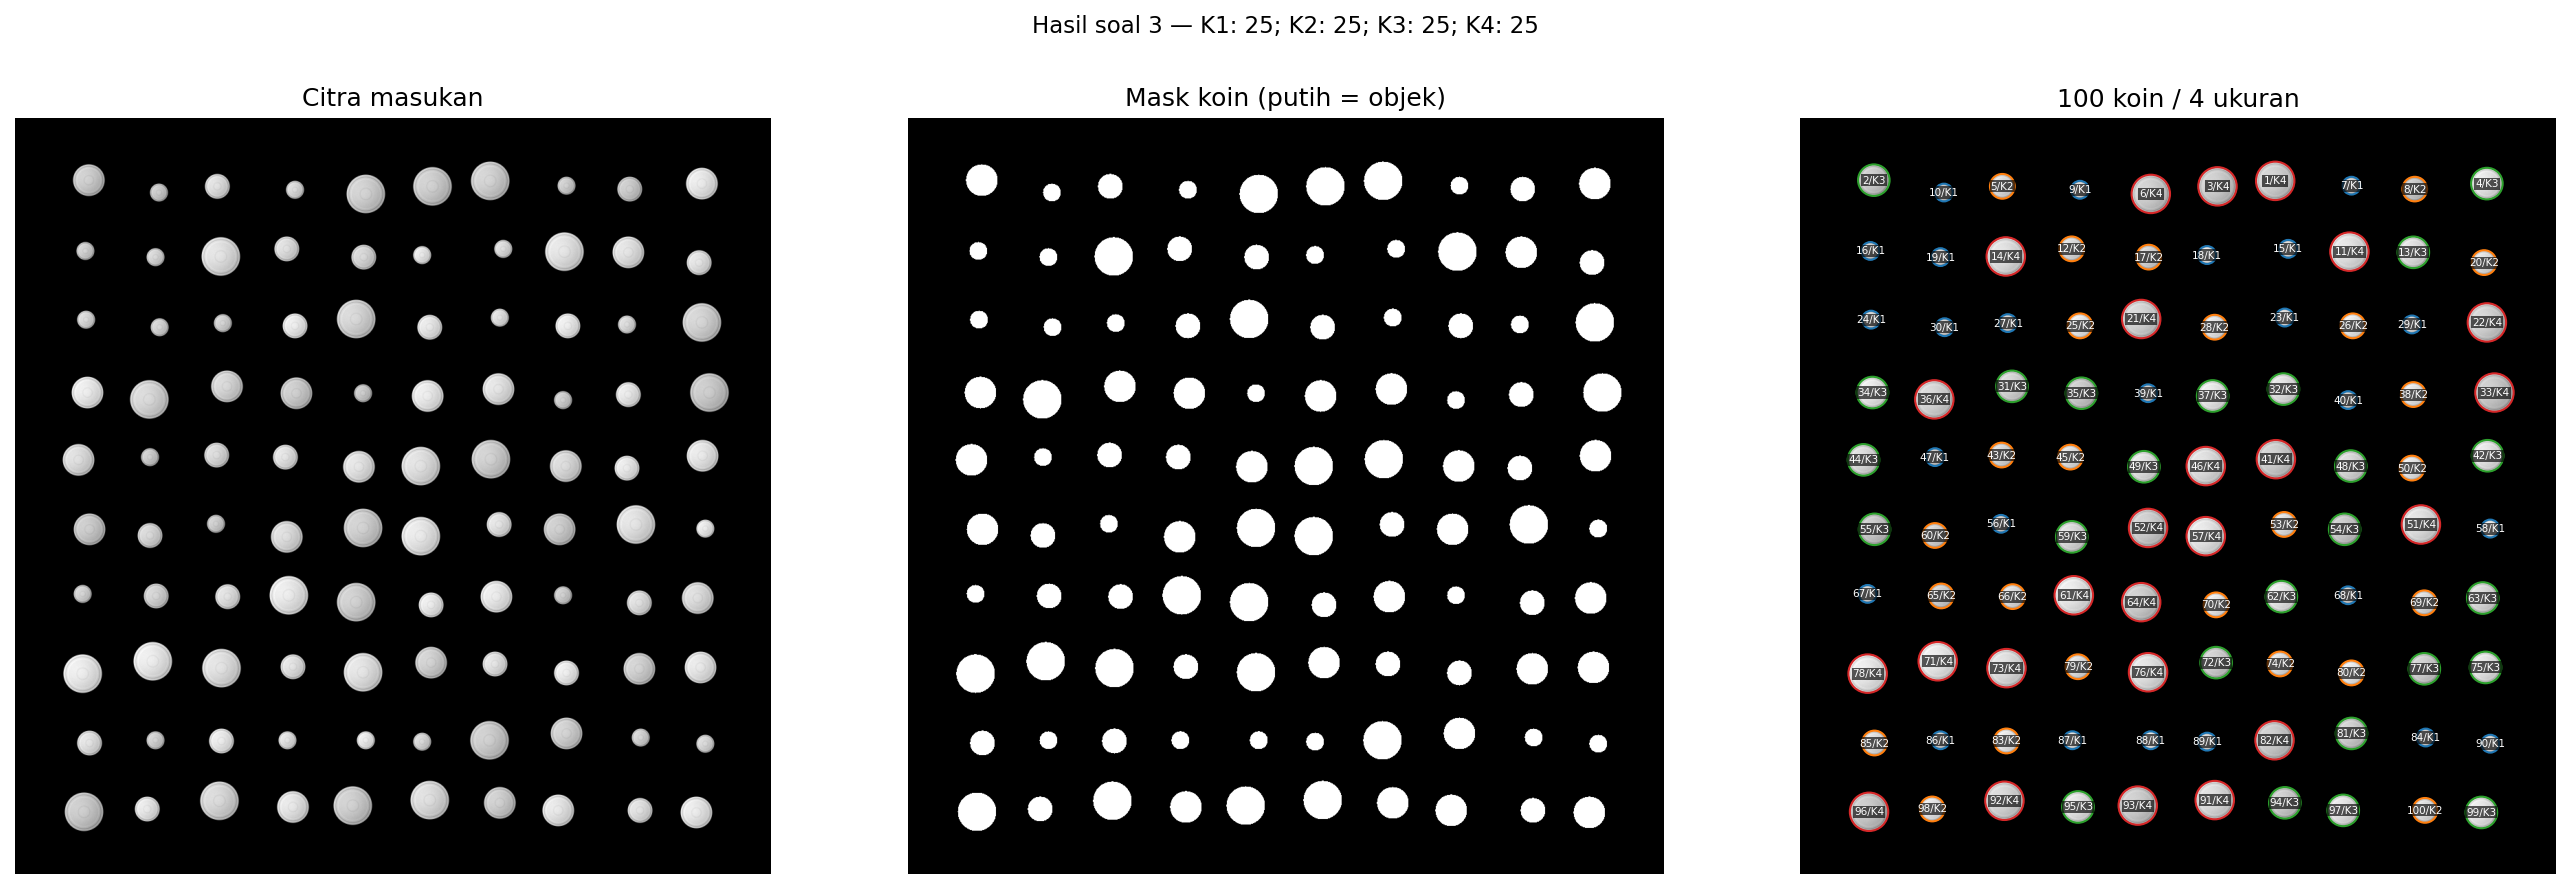
\includegraphics[width=\textwidth]{images/koin-ringkasan.png}
\caption{Citra sintetis, mask segmentasi, dan anotasi hasil.
Tulisan ID/K menunjukkan identitas objek dan kelompok ukurannya.}
\label{fig:koin-ringkasan}
\end{figure}

Jumlah dan distribusi ukuran sesuai dengan metadata pembangkit yang
diperiksa setelah deteksi. Perbedaan kecil antara diameter pembangkit dan
median hasil pengukuran timbul karena diskretisasi piksel, penghalusan
tepi pada citra sintetis, dan keputusan ambang segmentasi. Angka 100 pada
\kode{--expected-count} hanya digunakan untuk mengeluarkan peringatan
apabila jumlah hasil berbeda; parameter ini tidak menambah, menghapus,
atau membagi objek untuk mencapai jumlah tersebut. Statistik kelompok
dan peringatan disimpan pada \kode{ringkasan.json}; mask, label berwarna,
serta anotasi menyediakan bukti visual untuk memeriksa kesalahan.

\subsection{Batasan metode}

Koin bersentuhan dapat bergabung menjadi satu komponen, sedangkan koin
terpotong atau tertutup sebagian menghasilkan diameter yang terlalu
kecil. Pencahayaan tidak seragam, bayangan, dan latar bertekstur dapat
menurunkan mutu ambang global Otsu. Kesalahan pemilihan polaritas juga
mungkin terjadi apabila mayoritas bingkai bukan latar. Perbedaan
perspektif mengubah skala diameter antarlokasi, sementara dua ukuran
fisik yang sangat dekat dapat tergabung akibat toleransi 8\%.
Karena itu, hasil pada data sintetis ini menunjukkan keberhasilan pada
asumsi yang dinyatakan, dan belum membuktikan keandalan pada seluruh
foto koin nyata. Parameter luas minimum dan toleransi ukuran tetap
perlu diperiksa bersama mask dan anotasi ketika memakai citra lain.

\clearpage
\subsection{Pengembangan tambahan: foto dengan pencahayaan tidak merata}
\label{sec:koin-watershed}

Pengembangan ini menguji kondisi di luar asumsi latar seragam pada soal.
Metode utama tetap Otsu. Pilihan \kode{--method watershed} memakai gradien
Sobel sebagai peta batas dan penanda intensitas untuk memisahkan objek
dari latar, mengikuti contoh resmi scikit-image~\cite{skimage-watershed}.
Setelah normalisasi dan penyesuaian polaritas agar objek terang, piksel
dengan intensitas di bawah $0{,}12$ menjadi penanda latar dan piksel di atas
$0{,}6$ menjadi penanda objek. Watershed menentukan kelas piksel sisanya.
Ambang tersebut merupakan parameter awal untuk foto uji, dapat disesuaikan
melalui \kode{--marker-low} dan \kode{--marker-high}, dan tidak berlaku
universal. Pengisian lubang, filter luas, pengukuran \kode{regionprops},
serta pengelompokan ukuran mengikuti tahap berikutnya yang sama.

Foto \kode{skimage.data.coins()} berisi 24 koin, berukuran
$303\times384$ piksel, dan berasal dari koleksi Brooklyn Museum menurut
dokumentasi scikit-image~\cite{skimage-coins}. Foto ini merupakan
\textbf{uji tambahan, bukan pengganti citra utama 100 koin}.

\begin{figure}[H]
\centering
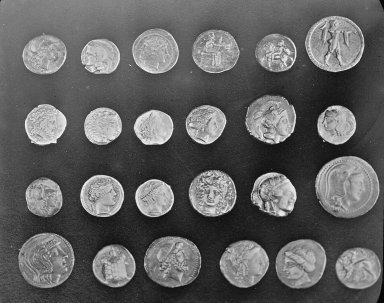
\includegraphics[width=0.31\textwidth]{images/koin-foto-nyata.png}\hfill
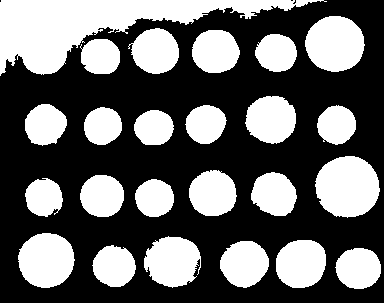
\includegraphics[width=0.31\textwidth]{images/koin-mask-otsu.png}\hfill
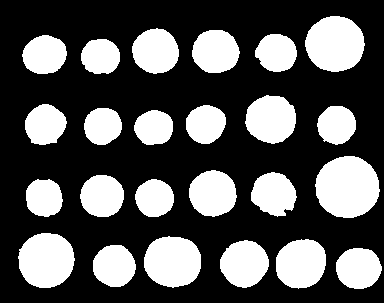
\includegraphics[width=0.31\textwidth]{images/koin-mask-watershed.png}
\caption{Dari kiri: foto asli, mask Otsu, dan mask watershed. Pada Otsu,
koin kiri atas menyatu dengan latar terang; watershed memisahkannya.}
\end{figure}

Kedua metode menghasilkan 24 region. Namun, jumlah yang sama tidak
menjamin segmentasi benar. Pada Otsu, satu region menggabungkan koin kiri
atas dengan latar, menghasilkan diameter ekuivalen sekitar $109{,}62$ piksel.
Pada watershed, 24 pusat acuan yang ditandai secara visual masing-masing
berada pada region berbeda, dengan selisih centroid kurang dari 3 piksel;
seluruh kotak pembatas juga terpisah dari bingkai. Ini memeriksa lokasi
dan identitas objek, bukan ketepatan setiap piksel mask atau diameter fisik.
Lima kelompok diameter piksel berjumlah 10, 8, 2, 3, dan 1; kelompok
tersebut belum divalidasi sebagai kategori ukuran fisik atau nominal uang.

\begin{lstlisting}[style=terminal]
.\.venv\Scripts\python.exe soal3/main.py --input soal3/data/koin_nyata_scikit.png --method watershed --expected-count 24 --output-dir soal3/hasil_foto_nyata_watershed
\end{lstlisting}

Pemeriksaan tambahan mencakup foto ini serta citra dengan gradien latar
dan inversi intensitas. Metode tetap memerlukan penanda yang sesuai dan
koin terpisah; belum menjamin keberhasilan pada semua pencahayaan atau
latar bertekstur. Pada metode bawaan, mask dan CSV pengukuran 100 koin
sintetis tetap identik dengan hasil sebelum pengembangan.
